
\section{Leveling Up}
\label{Section_Leveling}
After completing an encounter, your character has experienced a lot, and is ready to level up. You may choose \textbf{one new class} and add it to your tableau.

\textbf{Restrictions} 
\begin{itemize}
	\item \textbf{Rank 1} -  Any \textbf{new} class, no duplicates.
	\item \textbf{Rank 2} - To choose a rank 2 class, you must already \textbf{possess the rank 1} class.	
\end{itemize}

After slotting the new class tile into your tableau, take the \textbf{cards} of that class, and increase your starting \textbf{life} by the amount stated on the new class. Remember to use your new \textbf{passive}, when it comes up. You always add new classes, and you never loose passives, life, dice or cards you have gained before.

\textbf{Deckbuilding} Your action deck consists of exactly \textbf{16 cards}. When you put new cards in, you must remove an equal amount. You keep all the cards you acquire at your disposal, and you may return them to your deck later - but a card will have to be removed for each old one going back into your deck. 

\begin{tcolorbox}[colframe=red, colback=white]
	Important - Usually every class comes with one passive, 5 cards and around 3 starting life.
\end{tcolorbox} 

\section{Strategy Guide}
\label{Section_Strategy}

\textbf{Multiclassing} - The large amount of options you have allow you to push your deck and playstyle in vastly different directions. Character builds are also quite malleable, as half of your classes are decided after you already have some fighting experience.

\textbf{Co-Operation} - With more players on the table come more options on how to synergise and sequence your cards.

\textbf{Deck Thinning} -  Some passives and events let you reduce the number of cards in your deck. While more is often better in life, this is untrue in Deckbuilders. You generally want to use your strongest cards as often as possible, and removing weaker ones increases the frequency with which you can find them.


\newpage

\section{Optional Rules}
\label{Section_OptionalRules}

\subsection*{Events} 

\begin{figure}[ht]
	\begin{minipage}[t][6.5cm][t]{0.5\textwidth}
		If you want to add some more variety to the game, you can add events.
		
		After every encounter, your can draw an event. These will change how you play the rest of the story. All events have an  \textbf{upside} and a  \textbf{downside} which will affect your choices and gameplay.
		
		Some events will make the game harder, and some easier. Some will warp your choices around them, and some may barely affect you. The only guarantee is that no two stories will play out the same.
		
		Events stay active \textbf{for the entire story}.
	\end{minipage}	
	\begin{minipage}[t][6.5cm][t]{0.5\textwidth}
		\centering
		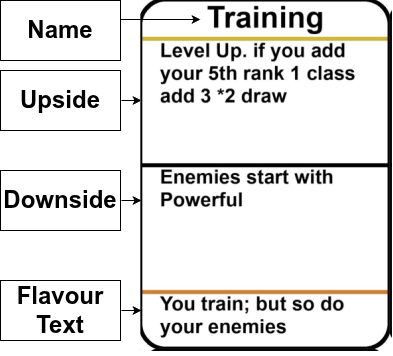
\includegraphics[width=0.9\linewidth, valign=t]{../ExplanationPics/Event.drawio.png}
	\end{minipage}
\end{figure}
\begin{tcolorbox}[colframe=blue, colback=white]
	Reminder - Events happen before the level up.
\end{tcolorbox}


\textbf{Quick play:} If you are short on time, you can play a single encounter instead of a whole story. Instead of the normal setup, choose a single encounter of the story you want to play. Level up and draw events as you normally would on the way to the chosen encounter, but skip all combat. After completing the encounter, you may continue as normal or end the session. %TODO check with publisher whether this is good on a spiritual evel.

\textbf{Hardcore backlined:} If you need a more intense experience, you can change the backlined state to mean that you do not get to play any cards and you passives no longer apply. Essentially, a backlined player no longer participates in the fight at all.

\textbf{Sequential Turns:}  If you find it very hectic for all players to take the turns simultaneously, you can choose to play one player at a time. In this case it may be nice for all players to look at the current players hand and discuss.

\textbf{Even more simultaneous turns:}  If you need a very hectic experience, don't synchronise your turns. Just play your cards as fast as you can, act for and rotate the enemies when you finish. This is not very balanced. The player that killed the most enemies wins. Try snatching elements whenever possible, it improves your K/D.
 


